

\tikzset{every picture/.style={line width=0.75pt}} %set default line width to 0.75pt        

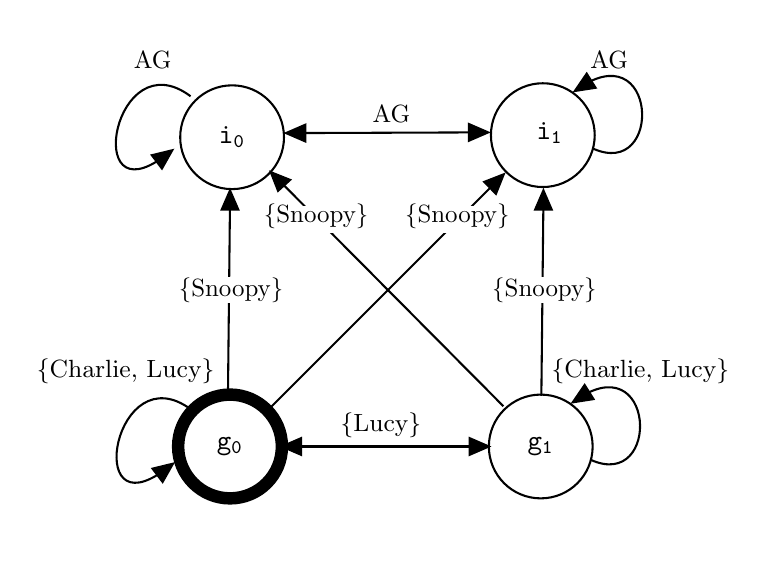
\begin{tikzpicture}[x=0.75pt,y=0.75pt,yscale=-1,xscale=1]
%uncomment if require: \path (0,300); %set diagram left start at 0, and has height of 300

%Curve Lines [id:da6922101751426857] 
\draw    (326.43,51.72) .. controls (366.43,21.72) and (369.63,95.32) .. (334.83,79.32) ;


%Curve Lines [id:da6315070066186073] 
\draw    (141.29,54.27) .. controls (104.49,26.67) and (88.76,113.08) .. (128.76,83.08) ;


%Straight Lines [id:da0043984547546391806] 
\draw    (191.92,72) -- (280.03,71.67) ;


%Straight Lines [id:da8170776057111964] 
\draw    (311.29,104.28) -- (310.29,198.64) ;


%Straight Lines [id:da10125059076875131] 
\draw    (288.88,95.12) -- (177.9,206.1) ;


%Straight Lines [id:da13591440442801073] 
\draw    (183.13,94.02) -- (292,203.6) ;


%Curve Lines [id:da0862450190271058] 
\draw    (141.62,205.27) .. controls (104.82,177.67) and (89.1,264.08) .. (129.1,234.08) ;


%Straight Lines [id:da17405321396390305] 
\draw    (160.29,104.28) -- (159.29,198.64) ;


%Straight Lines [id:da018251469869151382] 
\draw    (185.29,223) -- (285,223) ;

%Curve Lines [id:da8507870813478686] 
\draw    (325.43,201.72) .. controls (365.43,171.72) and (368.63,245.32) .. (333.83,229.32) ;

%Shape: Circle [id:dp9462184779936802] 
\draw   (286,73) .. controls (286,59.19) and (297.19,48) .. (311,48) .. controls (324.81,48) and (336,59.19) .. (336,73) .. controls (336,86.81) and (324.81,98) .. (311,98) .. controls (297.19,98) and (286,86.81) .. (286,73) -- cycle ;
%Shape: Circle [id:dp6359205424734804] 
\draw  [line width=4.5]  (135.29,223) .. controls (135.29,209.19) and (146.48,198) .. (160.29,198) .. controls (174.09,198) and (185.29,209.19) .. (185.29,223) .. controls (185.29,236.81) and (174.09,248) .. (160.29,248) .. controls (146.48,248) and (135.29,236.81) .. (135.29,223) -- cycle ;
%Shape: Circle [id:dp06782137726568571] 
%Shape: Circle [id:dp8938158972072578] 
\draw  [line width=0.75]  (135.29,223) .. controls (135.29,209.19) and (146.48,198) .. (160.29,198) .. controls (174.09,198) and (185.29,209.19) .. (185.29,223) .. controls (185.29,236.81) and (174.09,248) .. (160.29,248) .. controls (146.48,248) and (135.29,236.81) .. (135.29,223) -- cycle ;
%Shape: Circle [id:dp19780391712041556] 
\draw   (285,223) .. controls (285,209.19) and (296.19,198) .. (310,198) .. controls (323.81,198) and (335,209.19) .. (335,223) .. controls (335,236.81) and (323.81,248) .. (310,248) .. controls (296.19,248) and (285,236.81) .. (285,223) -- cycle ;
%Shape: Triangle [id:dp4725710951486233] 
\draw  [fill={rgb, 255:red, 0; green, 0; blue, 0 }  ,fill opacity=1 ] (132.8,231.28) -- (127.82,240.08) -- (122.97,233.67) -- cycle ;
%Shape: Triangle [id:dp08394946096129607] 
\draw  [fill={rgb, 255:red, 0; green, 0; blue, 0 }  ,fill opacity=1 ] (285,223) -- (275.72,227.02) -- (275.72,218.98) -- cycle ;
%Shape: Triangle [id:dp12888926826248426] 
\draw  [fill={rgb, 255:red, 0; green, 0; blue, 0 }  ,fill opacity=1 ] (185.29,223) -- (194.56,218.98) -- (194.56,227.02) -- cycle ;
%Shape: Triangle [id:dp7536519811814515] 
\draw  [fill={rgb, 255:red, 0; green, 0; blue, 0 }  ,fill opacity=1 ] (325.43,201.72) -- (331.13,193.37) -- (335.42,200.17) -- cycle ;


\draw  [line width=0.75]  (136.29,74) .. controls (136.29,60.19) and (147.48,49) .. (161.29,49) .. controls (175.09,49) and (186.29,60.19) .. (186.29,74) .. controls (186.29,87.81) and (175.09,99) .. (161.29,99) .. controls (147.48,99) and (136.29,87.81) .. (136.29,74) -- cycle ;
%Shape: Triangle [id:dp8413979641210945] 
\draw  [fill={rgb, 255:red, 0; green, 0; blue, 0 }  ,fill opacity=1 ] (132.46,80.28) -- (127.49,89.08) -- (122.64,82.67) -- cycle ;
%Shape: Triangle [id:dp417855807516911] 
\draw  [fill={rgb, 255:red, 0; green, 0; blue, 0 }  ,fill opacity=1 ] (160.29,99.64) -- (164.3,108.92) -- (156.27,108.92) -- cycle ;
%Shape: Triangle [id:dp4971926593318259] 
\draw  [fill={rgb, 255:red, 0; green, 0; blue, 0 }  ,fill opacity=1 ] (292.17,91.86) -- (288.41,101.24) -- (282.75,95.53) -- cycle ;

%Shape: Triangle [id:dp5745677700051097] 
\draw  [fill={rgb, 255:red, 0; green, 0; blue, 0 }  ,fill opacity=1 ] (326.43,51.72) -- (332.13,43.37) -- (336.42,50.17) -- cycle ;

%Shape: Triangle [id:dp7023350686012408] 
\draw  [fill={rgb, 255:red, 0; green, 0; blue, 0 }  ,fill opacity=1 ] (284.67,71.67) -- (275.39,75.69) -- (275.39,67.65) -- cycle ;
%Shape: Triangle [id:dp6039108674849356] 
\draw  [fill={rgb, 255:red, 0; green, 0; blue, 0 }  ,fill opacity=1 ] (187.29,72) -- (196.56,67.98) -- (196.56,76.02) -- cycle ;
%Shape: Triangle [id:dp9176823524690971] 
\draw  [fill={rgb, 255:red, 0; green, 0; blue, 0 }  ,fill opacity=1 ] (179.93,90.84) -- (189.24,94.56) -- (183.44,99.82) -- cycle ;
%Shape: Rectangle [id:dp7039913742222839] 
\draw  [color={rgb, 255:red, 0; green, 0; blue, 0 }  ,draw opacity=0 ][fill={rgb, 255:red, 255; green, 255; blue, 255 }  ,fill opacity=1 ] (148.29,141.18) -- (173.29,141.18) -- (173.29,153.97) -- (148.29,153.97) -- cycle ;
%Shape: Triangle [id:dp2216172811102144] 
\draw  [fill={rgb, 255:red, 0; green, 0; blue, 0 }  ,fill opacity=1 ] (311.29,99.64) -- (315.3,108.92) -- (307.27,108.92) -- cycle ;
%Shape: Rectangle [id:dp8761718319086598] 
\draw  [color={rgb, 255:red, 0; green, 0; blue, 0 }  ,draw opacity=0 ][fill={rgb, 255:red, 255; green, 255; blue, 255 }  ,fill opacity=1 ] (299.29,141.18) -- (324.29,141.18) -- (324.29,153.97) -- (299.29,153.97) -- cycle ;
%Shape: Rectangle [id:dp30238976789343086] 
\draw  [color={rgb, 255:red, 0; green, 0; blue, 0 }  ,draw opacity=0 ][fill={rgb, 255:red, 255; green, 255; blue, 255 }  ,fill opacity=1 ] (257.29,107.18) -- (282.29,107.18) -- (282.29,119.97) -- (257.29,119.97) -- cycle ;
%Shape: Rectangle [id:dp8647257034518798] 
\draw  [color={rgb, 255:red, 0; green, 0; blue, 0 }  ,draw opacity=0 ][fill={rgb, 255:red, 255; green, 255; blue, 255 }  ,fill opacity=1 ] (189.29,107.18) -- (214.29,107.18) -- (214.29,119.97) -- (189.29,119.97) -- cycle ;

% Text Node
\draw (160.29,223) node  [align=left] {$\mathtt{g_0}$};
% Text Node
\draw (310,223) node  [align=left] {$\mathtt{g_1}$};
% Text Node
\draw (161.29,74) node  [align=left] {$\mathtt{i_0}$};
% Text Node
\draw (314.29,72) node  [align=left] {$\mathtt{i_1}$};
% Text Node
\draw (238,63) node [scale=0.9] [align=left] {\agentSlide{AG}};
% Text Node
\draw (123,37) node [scale=0.9] [align=left] {\agentSlide{AG}};
% Text Node
\draw (343,37) node [scale=0.9] [align=left] {\agentSlide{AG}};
% Text Node
\draw (160.79,147.58) node [scale=0.9] [align=left] {\{\agentSlide{Snoopy}\}};
% Text Node
\draw (311.79,147.58) node [scale=0.9] [align=left] {\{\agentSlide{Snoopy}\}};
% Text Node
\draw (269.79,112.18) node [scale=0.9] [align=left] {\{\agentSlide{Snoopy}\}};
% Text Node
\draw (201.79,112.18) node [scale=0.9] [align=left] {\{\agentSlide{Snoopy}\}};
% Text Node
\draw (110,186.6) node  [align=left] {{\small \{\agentSlide{Charlie}, \agentSlide{Lucy}\}}};
% Text Node
\draw (358,186.6) node  [align=left] {{\small \{\agentSlide{Charlie}, \agentSlide{Lucy}\}}};
% Text Node
\draw (233,212.6) node  [align=left] {{\small \{\agentSlide{Lucy}\}}};
% Text Node
%\draw (230,33.07) node [scale=0.9] [align=left] {\agentSlide{AG} = \{\agentSlide{Charlie}, \agentSlide{Lucy}, \agentSlide{Snoopy}\}};


\end{tikzpicture}